\section{Virtual Organization Over NDN}

To facilitate explanation, in this section, we will use the following example (Figure) to illustrate the VO system.
There are two real-world organizations in our example: UCLA and MIT.
Both UCLA and MIT will produce networking lecture data and Number-theory lecture data.
There are also two VOs containing networking lecture data names and number theory lecture data names respectively.
In this way, the authorised consumers could easily access the networking/number theory lecture data both from UCLA and MIT through VO.

\begin{figure*}[t]
  \centering
  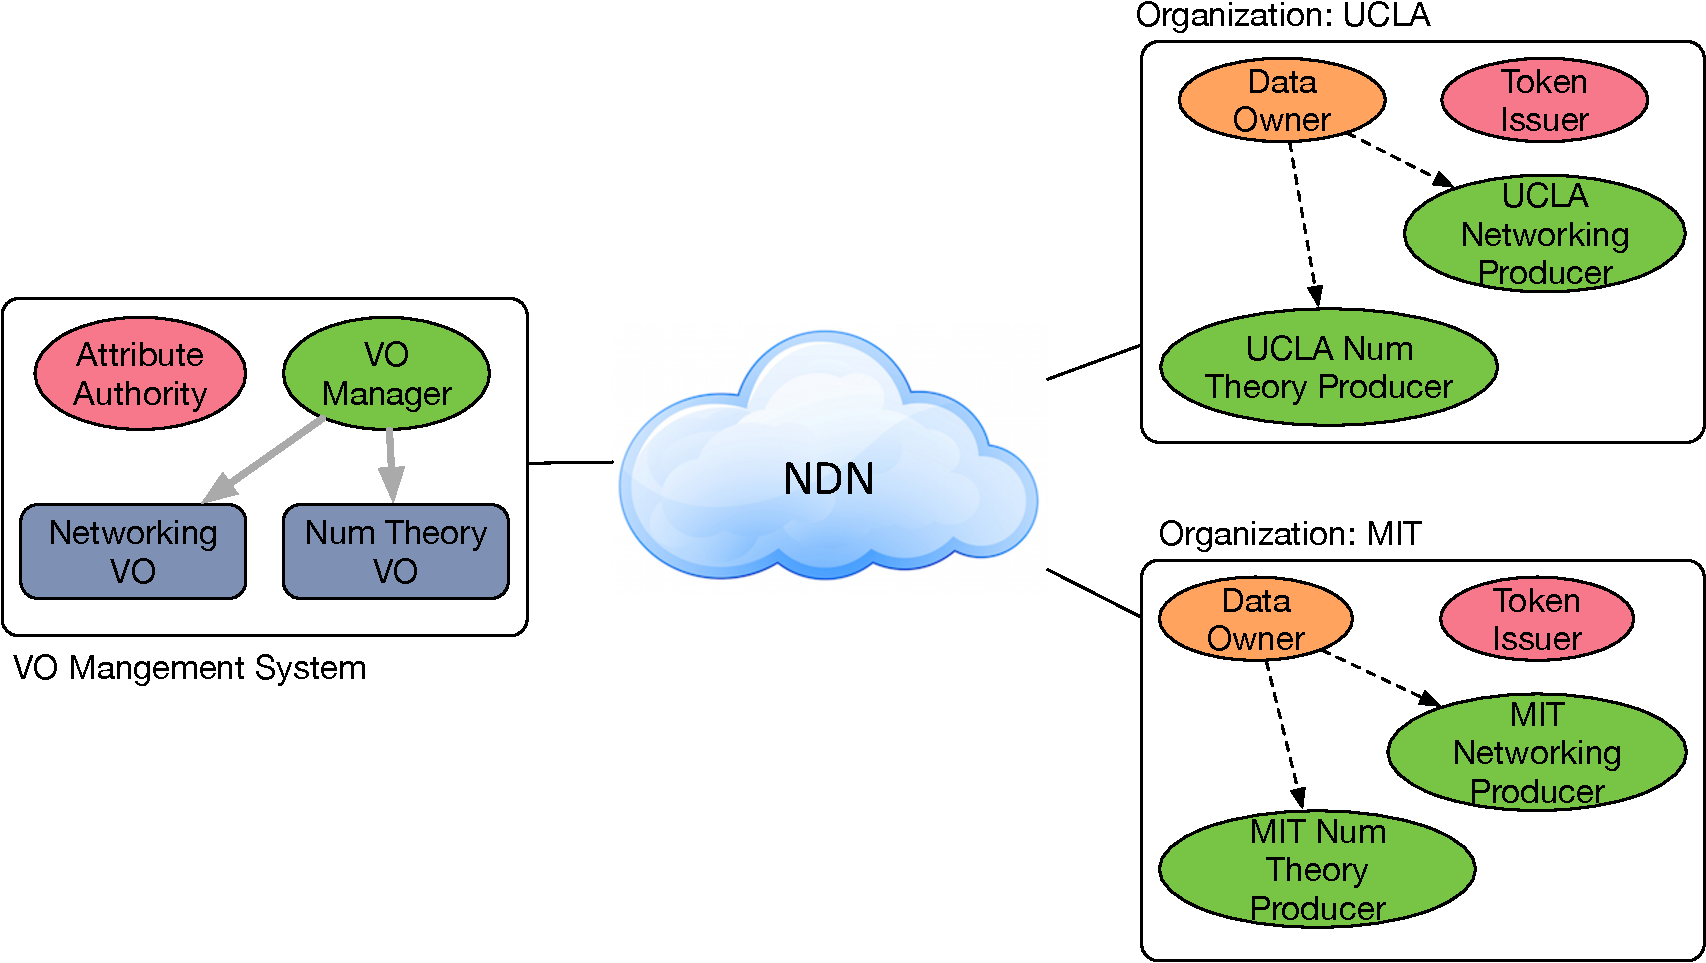
\includegraphics[scale=0.5]{figures/example}
  \vspace{-3mm}
  \caption{An example of how VO system work}
  \label{fig:example}
\end{figure*}

\subsection{VO Mangement System}

\subsubsection{Attribute Authority}

\subsubsection{VO Manager}


\subsection{Organization}

\subsubsection{Producer}

\subsubsection{Data Owner}

\subsubsection{Token Issuer}


\subsection{Consumer}